\chapter{Thực nghiệm}

Chương này trình bày các kết quả thực nghiệm nhằm giải quyết các câu hỏi nghiên cứu của khóa luận, bao gồm: so sánh điều khiển vòng kín F0 và F1 trên LIBERO-Mem, kiểm tra cơ chế truy vấn theo sự kiện, phân tích hiện tượng overshoot, can thiệp triệt tiêu bộ nhớ, và đánh giá khả năng duy trì kỹ năng cơ sở trên LIBERO-10. Các thử nghiệm được tiến hành trên hai mô hình nền là SmolVLA \cite{smolvla2025} và X-VLA \cite{xvla2025}. Bảng~\ref{tab:experiment-rq-map} tóm tắt năm nhóm thực nghiệm trọng tâm, quy mô mẫu và mục tiêu khoa học tương ứng với từng câu hỏi nghiên cứu.

\begin{table}[htbp]
\centering\small
\caption{Tổng hợp các nhóm thực nghiệm trọng tâm theo mục tiêu và câu hỏi nghiên cứu}
\label{tab:experiment-rq-map}
\setlength{\tabcolsep}{4pt}
\begin{tabular}{>{\raggedright\arraybackslash}p{\dimexpr 0.24\textwidth-2\tabcolsep\relax}|>{\raggedright\arraybackslash}p{\dimexpr 0.18\textwidth-2\tabcolsep\relax}|>{\raggedright\arraybackslash}p{\dimexpr 0.23\textwidth-2\tabcolsep\relax}|>{\raggedright\arraybackslash}p{\dimexpr 0.345\textwidth-2\tabcolsep\relax}}
\toprule
\textbf{Nhóm thực nghiệm} & \textbf{Mô hình áp dụng} & \textbf{Quy mô mẫu} & \textbf{Mục tiêu khoa học \& RQ} \\
\midrule
So sánh vòng kín F0 và F1 trên LIBERO-Mem & SmolVLA, X-VLA & 40 cặp ghép mỗi mô hình, 160 lượt & Đo lường tác động của bộ nhớ sự kiện lên SR và SCR (RQ1) \\
\midrule
Truy vấn theo sự kiện và lỗi overshoot & SmolVLA, X-VLA & 24 cặp ghép mỗi mô hình, 96 lượt & Kiểm tra cơ chế truy vấn sớm và mô tả hiện tượng overshoot (RQ2) \\
\midrule
Cơ chế dừng ngoại vi dựa trên bộ nhớ & X-VLA & 35 mốc, 60 lượt mô phỏng can thiệp dừng, 40 + 24 lượt vòng kín & Đo khả năng khắc phục overshoot bằng tín hiệu dừng dựa trên bộ nhớ (RQ2) \\
\midrule
Can thiệp xóa bỏ truy vấn & SmolVLA, X-VLA & 3 ca can thiệp, mỗi ca một nhánh đối chứng & Đo độ nhạy cục bộ của hành động với lời nhắc bộ nhớ (RQ1) \\
\midrule
Duy trì kỹ năng cơ sở trên LIBERO-10 & SmolVLA, X-VLA & 50 bộ ba ghép cặp mỗi mô hình, 300 lượt & Đánh giá mức độ suy giảm kỹ năng gốc và quên thảm khốc (RQ3) \\
\bottomrule
\end{tabular}
\end{table}

\section{Thiết lập thực nghiệm và chỉ số đánh giá}

\label{sec:conditions}

\subsection{Kiểm chứng tái lập trạng thái cảnh}
\label{sec:reproduction-scene}

Việc khôi phục trạng thái ban đầu và để cảnh ổn định là một phần của quy trình đánh giá. Mã nguồn LIBERO-Mem công bố các phụ thuộc cho bước thu thập dữ liệu, trong đó có MuJoCo 3.2.2 và phiên bản robosuite đi kèm; hướng dẫn cũng ghi nhận một số quỹ đạo có thể phát lại không thành công dù dùng cùng trạng thái ban đầu và hạt giống \cite{liberomemSource}. Phiên bản thư viện được khai báo trong mã nguồn cung cấp cơ sở dựng môi trường, còn tệp demonstration được kiểm tra không ghi phiên bản hoặc bản dựng MuJoCo đã thực sự tạo ra dữ liệu đó.

Để kiểm tra trạng thái cảnh trước khi chính sách hoạt động, nghiên cứu phát lại riêng \texttt{demo\_33} của tác vụ T1 với mã nguồn LIBERO-Mem đã khóa phiên bản, robosuite 1.4.1 đi kèm và MuJoCo 3.2.2; Python 3.10.22 là lựa chọn của nghiên cứu. Phép kiểm tra dùng robot Panda, bộ điều khiển OSC\_POSE và tần số 20 Hz. Vector trạng thái lấy từ metadata của demonstration được khôi phục với sai số tuyệt đối cực đại bằng 0, sau đó môi trường thực hiện 20 hành động khởi động theo quy trình tinh chỉnh dữ liệu của tác giả. Chai rượu trong cảnh ban đầu đứng thẳng, nghiêng quá $90^\circ$ ở bước 13 và đạt khoảng $107{,}26^\circ$ ở bước 20. Trong khung hình đầu tiên của demonstration đã tinh chỉnh, chai vẫn đứng thẳng như Hình~\ref{fig:bottle-replay}. Quan sát ảnh được đối chiếu sau khi áp dụng phép biến đổi hướng ảnh của tác giả; tệp demonstration không cung cấp tư thế vật lý của chai để so sánh định lượng trực tiếp.

\begin{figure}[H]
\centering
\begin{tabular}{cc}
\includegraphics[width=.34\linewidth]{figures/tai-lap-chai-replay.png} &
\includegraphics[width=.34\linewidth]{figures/tai-lap-chai-cong-bo.png} \\
(a) Phát lại sau 20 bước & (b) Khung hình đầu công bố
\end{tabular}
\caption{Tư thế chai trong phép kiểm chứng T1 \texttt{demo\_33} và demonstration LIBERO-Mem đã tinh chỉnh.}
\label{fig:bottle-replay}
\end{figure}

Sai khác được ghi nhận trước hành động đầu tiên của policy trong episode được kiểm tra. Nguyên nhân cụ thể chưa được xác định; sự khác biệt về môi trường mô phỏng hoặc điều kiện tạo dữ liệu là các khả năng cần kiểm chứng thêm. Hình học vật thể, tiếp xúc và chuỗi hành động khởi động được giữ nguyên trong phép kiểm tra. Cấu hình chẩn đoán này được dựng riêng để đối chiếu nguồn tác giả; cấu hình của các thực nghiệm vòng kín được mô tả trong các mục tương ứng.

Nhằm bóc tách ảnh hưởng của từng thành phần kiến trúc, nghiên cứu thiết lập bốn điều kiện về mô hình như tổng hợp tại Bảng~\ref{tab:experimental-conditions}.

\begingroup\small\setlength{\tabcolsep}{4pt}\renewcommand{\arraystretch}{1.15}
\begin{longtable}{>{\raggedright\arraybackslash}p{\dimexpr 0.17\textwidth-2\tabcolsep\relax}|>{\raggedright\arraybackslash}p{\dimexpr 0.25\textwidth-2\tabcolsep\relax}|>{\raggedright\arraybackslash}p{\dimexpr 0.25\textwidth-2\tabcolsep\relax}|>{\raggedright\arraybackslash}p{\dimexpr 0.30\textwidth-2\tabcolsep\relax}}
\caption{Các cấu hình thực nghiệm}\label{tab:experimental-conditions}\\
\toprule
\textbf{Điều kiện} & \textbf{Trọng số mô hình} & \textbf{Ngữ cảnh văn bản} & \textbf{Mục đích đánh giá} \\
\midrule\endfirsthead
\toprule
\textbf{Điều kiện} & \textbf{Trọng số mô hình} & \textbf{Ngữ cảnh văn bản} & \textbf{Mục đích đánh giá} \\
\midrule\endhead
\bottomrule\endfoot
B0 & Checkpoint gốc & Chỉ dẫn gốc & Mốc tham chiếu nền tảng trước thích ứng \\
F0 & Adapter LoRA thường & Chỉ dẫn gốc & Đo lường tác động của thích ứng không bộ nhớ \\
F1 & Adapter LoRA có bộ nhớ & Chỉ dẫn kèm sự kiện & Đánh giá hiệu quả của phương pháp đề xuất \\
F1-off & Trọng số của F1 & Chỉ dẫn gốc & Kiểm tra độ nhạy và sự phụ thuộc vào bộ nhớ \\
\end{longtable}
\endgroup

Khi có thông tin hợp lệ từ bộ nhớ, F1 nhận chuỗi dữ kiện vào sau chỉ dẫn gốc, bắt đầu với tiền tố \texttt{Memory:}. Hình~\ref{fig:prompt-example} minh họa cấu trúc lời nhắc tại bước khởi tạo và bước 312 khi bộ nhớ ghi nhận chu kỳ hoàn trả bát kèm chỉ báo \texttt{History incomplete.} khi lịch sử quan sát chưa bảo đảm tính đầy đủ.

\begin{figure}[htbp]
\centering
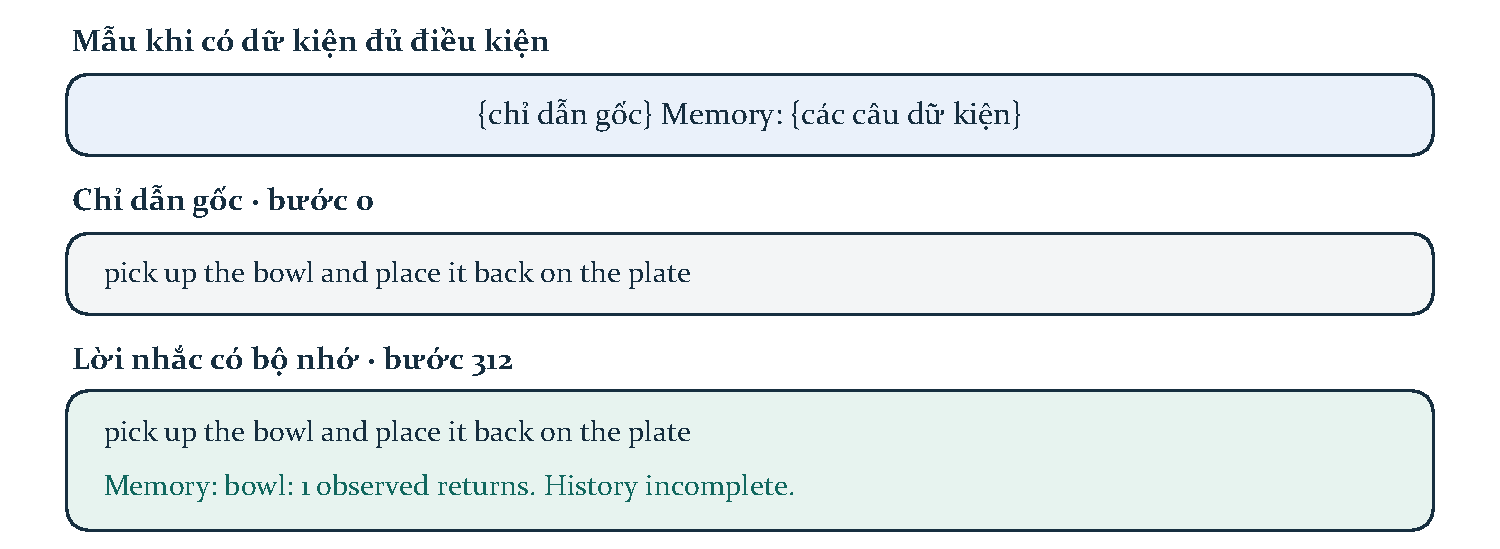
\includegraphics[width=.96\linewidth]{figures/loi-nhac-bo-nho.pdf}
\caption{Cấu trúc lời nhắc tích hợp bộ nhớ và ví dụ thực tế từ lượt chạy T1}
\label{fig:prompt-example}
\end{figure}

\label{sec:xvla-setup}

Để kiểm chứng tính tổng quát của phương pháp bộ nhớ sự kiện có bằng chứng theo RQ3, nghiên cứu triển khai song song quy trình thích ứng và đánh giá trên hai kiến trúc mô hình nền tiêu biểu: SmolVLA \cite{smolvla2025} và X-VLA \cite{xvla2025}. Bảng~\ref{tab:model-comparison} tổng hợp và so sánh chi tiết các thông số kỹ thuật và thiết lập điều khiển giữa hai mô hình. Trong khi SmolVLA dự đoán đoạn hành động độ dời tương đối $H = 50$ bước qua action expert nhỏ gọn, X-VLA dự đoán tư thế tuyệt đối 6D của đầu gắp với đoạn $H = 30$ bước qua 10 bước biến đổi Flow Matching trên nền tảng Florence-2. Cả hai mô hình đều vận hành ở nhịp truy vấn định kỳ $s = 10$ bước và chia sẻ cùng phân phối dữ liệu tinh chỉnh có bộ nhớ, với ngân sách thích ứng tham số lần lượt là 645.120 tham số LoRA trên SmolVLA và khoảng 11,87 triệu tham số trên X-VLA (5.000 bước huấn luyện, kích thước lô 32, tốc độ học $5\times10^{-5}$).

\begin{table}[htbp]
\centering\small
\caption{So sánh thông số kỹ thuật và thiết lập điều khiển giữa SmolVLA và X-VLA}
\label{tab:model-comparison}
\setlength{\tabcolsep}{4pt}
\begin{tabular}{>{\raggedright\arraybackslash}p{\dimexpr 0.28\textwidth-2\tabcolsep\relax}|>{\raggedright\arraybackslash}p{\dimexpr 0.36\textwidth-2\tabcolsep\relax}|>{\raggedright\arraybackslash}p{\dimexpr 0.36\textwidth-2\tabcolsep\relax}}
\toprule
\textbf{Thông số / Thuộc tính} & \textbf{SmolVLA} & \textbf{X-VLA} \\
\midrule
Checkpoint gốc & \texttt{lerobot/smolvla\_libero} & \texttt{2toINF/X-VLA-Libero} \\
Kiến trúc VLM & SigLIP + SmolLM2 & Florence-2-large \\
Không gian hành động & Độ dời tương đối 7D ($\Delta$ pose + kẹp) & Tư thế tuyệt đối 6D + kẹp \\
Bộ điều khiển robot & OSC (\textit{use\_delta} = True) ở 20 Hz & OSC (\textit{use\_delta} = False) ở 20 Hz \\
Đầu vào ảnh mô hình & $2 \times (256 \times 256)$ & $2 \times (224 \times 224)$ \\
Vector cảm nhận bản thể & 8D (vị trí, hướng xoay, kẹp) & 9D (vị trí, xoay 6D, kẹp; đệm) \\
Độ dài đoạn hành động ($H$) & 50 bước & 30 bước \\
Nhịp thực thi, truy vấn ($s$) & 10 bước định kỳ & 10 bước định kỳ \\
Tham số huấn luyện ($\phi$) & 645.120 tham số LoRA & $\sim 11{,}87$ triệu tham số \\
\bottomrule
\end{tabular}
\end{table}

Hiệu năng thực thi được lượng hóa qua ba chỉ số: chỉ số thành công toàn phần $S_i = \mathbf{1}[z_i = N \land P_i \land \neg O_i] \in \{0, 1\}$, trong đó $z_i$ là số chu kỳ xác nhận, $N$ là số chu kỳ yêu cầu, $P_i$ là vị từ kiểm tra đích, và $O_i$ là cờ vi phạm overshoot; tỷ lệ hoàn thành mốc $\mathrm{SCR}_i = z_i / N$; cùng tỷ lệ thành công thực nghiệm $\widehat{\mathrm{SR}} = \frac{1}{n}\sum_{i=1}^{n} S_i$ trên $n$ lượt đánh giá.

\section{Đối sánh vòng kín trên LIBERO-Mem}

Thực nghiệm trực tiếp với hai adapter F0 và F1 trên 20 trạng thái unseen của tác vụ một chu kỳ T1 và ba chu kỳ T3 cho thấy những sự khác biệt rõ rệt.
\begin{table}[htbp]
\centering\small
\caption{So sánh hiệu năng vòng kín giữa F0 và F1 trên SmolVLA và X-VLA (40 cặp unseen)}
\label{tab:e2-comparison}
\label{tab:e2-unseen-results}
\label{tab:xvla-e2-results}
\setlength{\tabcolsep}{4.5pt}
\begin{tabular}{l|l|l|r|r|r|r}
\toprule
\textbf{Kiến trúc} & \textbf{Tác vụ} & \textbf{Điều kiện} & \shortstack{\textbf{Thành công}\\\textbf{(SR)}} & \shortstack{\textbf{SCR}\\\textbf{trung bình}} & \shortstack{\textbf{Vi phạm}\\\textbf{overshoot}} & \shortstack{\textbf{Không đạt}\\\textbf{mốc nào}} \\
\midrule
SmolVLA & T1 & F0 & 3/20 & 0,250 & 2/20 & 15/20 \\
        &    & F1 & 0/20 & 0,050 & 1/20 & 19/20 \\
        & T3 & F0 & 1/20 & 0,167 & 0/20 & 15/20 \\
        &    & F1 & 0/20 & 0,033 & 0/20 & 18/20 \\
        \cmidrule{2-7}
        & \textbf{Tổng} & \textbf{F0} & \textbf{4/40} & \textbf{0,208} & \textbf{2/40} & \textbf{30/40} \\
        &               & \textbf{F1} & \textbf{0/40} & \textbf{0,042} & \textbf{1/40} & \textbf{37/40} \\
\midrule
X-VLA   & T1 & F0 & 0/20 & 0,500 & 10/20 & 10/20 \\
        &    & F1 & 0/20 & 0,600 & 12/20 & 8/20 \\
        & T3 & F0 & 0/20 & 0,200 & 1/20 & 10/20 \\
        &    & F1 & 0/20 & 0,383 & 4/20 & 8/20 \\
        \cmidrule{2-7}
        & \textbf{Tổng} & \textbf{F0} & \textbf{0/40} & \textbf{0,350} & \textbf{11/40} & \textbf{20/40} \\
        &               & \textbf{F1} & \textbf{0/40} & \textbf{0,492} & \textbf{16/40} & \textbf{16/40} \\
\bottomrule
\end{tabular}
\end{table}

Bảng~\ref{tab:e2-comparison} cho thấy các adapter của hai họ mô hình thất bại theo hai cách khác nhau. Trên SmolVLA, chênh lệch tỷ lệ thành công giữa F1 và F0 là $10$ điểm phần trăm, với khoảng bootstrap 95\% từ $-20$ đến $-2{,}5$ điểm phần trăm. F1 chỉ đạt SCR trung bình $0{,}042$ so với $0{,}208$ của F0, và 37 trong 40 lượt F1 không đạt mốc nào. Một cách giải thích khả dĩ là adapter LoRA khoảng 645 nghìn tham số khó điều kiện hóa cả thông tin ngữ cảnh của môi trường LIBERO lẫn LIBERO-Mem để đưa ra hành động, dẫn đến năng lực thao tác cơ sở sụt giảm nghiêm trọng trên cả 2 lượt huấn luyện, thể hiện qua tỉ lệ đạt subgoal SCR trung bình chỉ từ $0{,}04$ đến $0{,}2$. Ngoài ra, việc chạy module bộ nhớ đồng thời với mô hình điều khiển trên phần cứng phổ thông làm trung vị thời gian mỗi lượt tăng từ 213 giây lên 1.066 giây. Với mô phỏng chạy đồng bộ, độ trễ này không ảnh hưởng đến kết quả, nhưng sẽ là một thách thức khi triển khai thực tế.

Trên X-VLA, F1 tăng SCR trung bình thêm $0{,}142$ so với F0 (từ $0{,}350$ lên $0{,}492$), nhưng cả hai đều đạt 0/40 vì tại mọi lượt hoàn thành đủ chu kỳ, mô hình điều khiển tiếp tục thực hiện thêm một chu kỳ nữa và bị tính là overshoot. Như vậy, ở X-VLA vấn đề chính không nằm ở việc hoàn thành chu kỳ mà ở việc dừng đúng lúc. Hai mô hình khác nhau ở nhiều điểm, gồm kích thước, số tham số được tinh chỉnh, biểu diễn hành động và checkpoint gốc, nên nghiên cứu không quy sự khác biệt về kết quả cho riêng một yếu tố nào. Cơ chế can thiệp và hỗ trợ quyết định bằng bộ nhớ ở mục sau sẽ giúp xử lý trực tiếp vấn đề này.

\section{Kiểm tra thực thi chuỗi hành động và hiện tượng overshoot}
\label{sec:d2-evidence}
\label{sec:d2-calibration}

Phân tích các trường hợp thất bại từ thực nghiệm đối sánh vòng kín trên LIBERO-Mem cho thấy một nguyên nhân đáng chú ý: việc robot thực thi cố định toàn bộ đoạn hành động sinh ra từ chính sách có nguy cơ bám theo các quyết định đã lỗi thời khi môi trường vật lý đã chuyển pha thao tác. Cơ chế điều phối truy vấn theo sự kiện được đề xuất nhằm giải quyết vấn đề này. Bộ điều phối liên tục giám sát trạng thái bộ nhớ sự kiện; ngay khi xuất hiện biến cố chuyển tiếp vật lý có bằng chứng xác nhận, hệ thống chủ động ngắt đoạn hành động đang thực thi dở dang và kích hoạt mô hình VLA tái truy vấn sớm với ngữ cảnh ngôn ngữ cập nhật.

Hình~\ref{fig:smolvla-chunk-failure} minh họa một trường hợp thất bại điển hình của SmolVLA trên tác vụ T1 khi thực thi cố định đoạn hành động ở chế độ giám sát ngầm. Sau khi tiếp cận bát ở bước 110, robot tiếp tục thực thi chuỗi hành động mở đã hoạch định trước. Tuy nhiên, sai lệch tiếp xúc khiến bát trượt khỏi đầu kẹp tại bước 142. Do không có cơ chế ngắt sớm để tái truy vấn theo biến cố nhận thức, robot vẫn thực thi trọn vẹn quỹ đạo nâng lên, dẫn đến việc tay kẹp nâng rỗng lên không trung tại bước 240 trong khi bát vẫn nằm nguyên trên đĩa. Thất bại này làm nổi bật sự cần thiết của cơ chế điều phối linh hoạt, cho phép ngắt sớm chuỗi hành động khi xuất hiện bằng chứng chuyển pha vật lý để tái lập kế hoạch kịp thời.

\begin{figure}[H]
\centering
\includegraphics[width=\linewidth]{figures/smolvla-chunk-failure.png}
\caption{Chuỗi hành vi thất bại của SmolVLA khi thực thi đoạn hành động}
\label{fig:smolvla-chunk-failure}
\end{figure}

Để kiểm chứng tính đúng đắn và hiệu quả của cơ chế này theo RQ2, nghiên cứu thiết lập thực nghiệm đối đầu trực tiếp giữa hai chế độ điều phối. Ở chế độ giám sát ngầm, bộ điều phối chỉ thụ động ghi nhận sự kiện vào bộ nhớ mà không can thiệp vào chu kỳ điều khiển, duy trì nghiêm ngặt nhịp truy vấn định kỳ $s = 10$ bước. Ngược lại, ở chế độ theo sự kiện, bộ điều phối được cấp quyền ngắt sớm đoạn hành động ngay khi có bằng chứng sự kiện mới để gọi lại chính sách trước hạn.

Quy trình đánh giá được thực hiện đồng nhất trên cả hai kiến trúc mô hình với cùng seed 42, khảo sát 12 trạng thái seen thuộc nhóm phát triển trên cả hai tác vụ T1 và T3. Với mỗi mô hình, thực nghiệm gồm 24 lượt ở chế độ theo sự kiện đối đầu ghép cặp với 24 lượt ở chế độ giám sát ngầm, tương ứng 48 lượt chạy vòng kín độc lập cho từng kiến trúc và tổng cộng 96 lượt đánh giá. Bảng~\ref{tab:d2-combined} tổng hợp kết quả đối sánh chi tiết giữa hai chế độ trên cả hai mô hình.

\begin{table}[htbp]
\centering\footnotesize
\caption{Đánh giá cơ chế truy vấn theo sự kiện và hiện tượng overshoot trên SmolVLA và X-VLA}
\label{tab:d2-combined}
\label{tab:d2-decision-results}
\label{tab:d2-calibration-results}
\setlength{\tabcolsep}{3.5pt}
\begin{tabular}{l|l|l|r|r|r|r|r}
\toprule
\textbf{Mô hình} & \textbf{Tác vụ} & \textbf{Chế độ} & \shortstack{\textbf{Thành}\\\textbf{công}} & \shortstack{\textbf{SCR}\\\textbf{TB}} & \shortstack{\textbf{Vi phạm}\\\textbf{overshoot}} & \shortstack{\textbf{Lần gọi}\\\textbf{VLA/lượt}} & \shortstack{\textbf{Lượt có}\\\textbf{gọi sớm}} \\
\midrule
SmolVLA & T1 & Giám sát & 1/12 & 0,167 & 1/12 & 94,33 & 0/12 \\
        &    & Theo sự kiện & 1/12 & 0,250 & 2/12 & 97,75 & 11/12 \\
        \cmidrule{2-8}
        & T3 & Giám sát & 0/12 & 0,056 & 0/12 & 100,00 & 0/12 \\
        &    & Theo sự kiện & 0/12 & 0,083 & 0/12 & 102,00 & 11/12 \\
\midrule
X-VLA   & T1 & Giám sát & 0/12 & 0,917 & 11/12 & 24,83 & 0/12 \\
        &    & Theo sự kiện & 0/12 & 0,833 & 10/12 & 31,92 & 11/12 \\
        \cmidrule{2-8}
        & T3 & Giám sát & 0/12 & 0,583 & 5/12 & 73,50 & 0/12 \\
        &    & Theo sự kiện & 0/12 & 0,528 & 4/12 & 78,00 & 11/12 \\
\bottomrule
\end{tabular}
\end{table}

Số liệu tại Bảng~\ref{tab:d2-combined} cho thấy cơ chế theo sự kiện vận hành hoàn toàn nhất quán về mặt kỹ thuật trên cả hai kiến trúc. Trên mỗi mô hình, có đúng 22 trên 24 lượt chạy ghi nhận ít nhất một lần kích hoạt ngắt sớm, gồm 11 trên 12 lượt ở tác vụ T1 và 11 trên 12 lượt ở tác vụ T3. Toàn bộ các lần gọi sớm này, gồm 56 lần ở SmolVLA và 70 lần ở X-VLA, đều xuất phát từ bằng chứng sự kiện mới được xác thực, chứng minh bộ điều phối phản ứng chính xác theo biến cố nhận thức thời gian thực chứ không kích hoạt ngẫu nhiên. Số lần gọi chính sách trung bình mỗi lượt ở chế độ theo sự kiện tăng nhẹ tương ứng với các thời điểm ngắt đoạn hành động trước hạn.

Mặc dù cơ chế ngắt sớm vận hành đúng thiết kế, tác động thực tế lên hiệu năng điều khiển vòng kín lại bộc lộ những đặc tính đối lập rõ rệt giữa hai họ mô hình:

Đối với SmolVLA, việc ngắt sớm đoạn hành động giúp cải thiện nhẹ tỷ lệ hoàn thành mốc SCR, tăng từ 0,167 lên 0,250 ở tác vụ T1 và từ 0,056 lên 0,083 ở tác vụ T3. Tuy nhiên, tỷ lệ thành công toàn phần không có sự bứt phá, duy trì ở mức 1 trên 12 lượt ở tác vụ T1 và 0 trên 12 lượt ở tác vụ T3 trên cả hai chế độ. Lượt T1 trạng thái 7 thành công ở bước 409 được minh họa tại Hình~\ref{fig:libero-mem-d2-t1-success} là một ví dụ trực quan đối lập với trường hợp thất bại ở Hình~\ref{fig:smolvla-chunk-failure}, cho thấy việc tái truy vấn đúng lúc giúp robot hoàn thành chuỗi thao tác kẹp nhấc và đặt bát. Dù vậy, việc ngắt sớm chỉ tối ưu hóa thời điểm cập nhật ngữ cảnh chứ không thể bù đắp được sự suy giảm năng lực vận động cơ sở sau thích ứng LoRA trên SmolVLA F1.

Trái ngược với SmolVLA, X-VLA thể hiện năng lực thao tác vật lý vượt trội khi đạt tỷ lệ hoàn thành mốc SCR rất cao ở cả hai chế độ, đạt từ 0,833 đến 0,917 ở tác vụ T1 và từ 0,528 đến 0,583 ở tác vụ T3. Tuy vậy, tỷ lệ thành công toàn phần của X-VLA vẫn là 0 trên 24 lượt ở cả hai chế độ. Nguyên nhân trực tiếp là phần lớn các lượt chạy đều thất bại do vi phạm lỗi overshoot. Sau khi hoàn thành thao tác đặt bát vào đĩa, mô hình tiếp tục quán tính sinh chuỗi hành động tiếp cận mới cho đến khi môi trường kết thúc lượt chạy. Ngay cả khi được ngắt action chunk và cho quan sát state mới, chính sách không phân biệt được trạng thái bắt đầu khi chưa thực hiện hành động và trạng thái kết thúc khi đã hoàn thành đủ lượt gắp.

\begin{figure}[H]
\centering
\includegraphics[width=\linewidth]{figures/t1-truy-van-som.png}\par
{\small\makebox[.25\linewidth]{Bước 0}%
\makebox[.25\linewidth]{Bước 142}%
\makebox[.25\linewidth]{Bước 409}%
\makebox[.25\linewidth]{Bước 1.000}\par}
\caption{Chuỗi hành vi của lượt T1 thành công khi kích hoạt truy vấn sớm}
\label{fig:libero-mem-d2-t1-success}
\end{figure}

\label{sec:xvla-d2-cohort}

Kết quả đối sánh vòng kín cùng thí nghiệm ngắt chuỗi hành động và truy vấn sớm trên cả hai mô hình giúp ta rút ra được một số quan sát: Việc ngắt chuỗi hành động action chunk và kích hoạt truy vấn sớm có thể tạo ra những đóng góp ý nghĩa nhất định, bằng chứng nằm ở cặp lượt chuyển từ False thành True tại task T1 state 7. Tuy nhiên việc ngắt sớm đoạn hành động và chuyển tiếp trạng thái cũng có thể thất bại, như state 5 của task T1 chuyển từ True sang False. Một quan sát khác là chỉ dẫn \texttt{Memory:...} không mang tính cưỡng chế để buộc chính sách VLA dừng lại khi đã hoàn thành nhiệm vụ. Bên cạnh đó, kết quả đo độ trễ của bộ ghi thị giác cho thấy độ trễ trung vị giữa thời điểm xác nhận được sự kiện và thời điểm diễn ra thực tế dao động từ 7 bước đến hàng chục bước, khiến thông tin ngôn ngữ luôn đến muộn hơn động học thực tế của robot và thay đổi của môi trường.

Ngoài ra, khảo sát ngoại tuyến trên các logged trace xác nhận việc nén ngân sách token xuống mức hai phần ba không làm suy hao dữ kiện bộ nhớ so với mức đầy đủ $B = 48$ token, với độ dài lời nhắc trung bình là 21 token ở tác vụ T1 và 26 token ở tác vụ T3. Khi rút xuống mức một phần ba, chỉ còn 35\% truy vấn ở T1 và 5,7\% truy vấn ở T3 giữ được dữ kiện. Vì mức hai phần ba và mức đầy đủ cho cùng kết quả truyền đạt dữ kiện, ngân sách $B = 48$ token không tạo ra điểm nghẽn biểu diễn trên các tác vụ khảo sát.

Sự hạn chế của chỉ dẫn ngôn ngữ trong việc ngăn chặn lỗi overshoot trên X-VLA là động lực trực tiếp dẫn đến thiết kế cơ chế hỗ trợ dừng thao tác dựa trên bộ nhớ được trình bày chi tiết tại Mục~\ref{sec:memory-halt}.

\section{Dừng thực thi dựa trên bộ nhớ trên X-VLA}
\label{sec:memory-halt}

Hiện tượng overshoot liên tục trên X-VLA cho thấy chính sách không có tín hiệu dừng sau khi hoàn thành nhiệm vụ. Thực nghiệm này sẽ khảo sát khả năng sử dụng bằng chứng từ bộ nhớ làm tín hiệu dừng ngoại vi. Quy trình sẽ bao gồm: đo độ nhạy của các phiên bản bộ nhớ trong việc phát hiện sự kiện, phân tích thời điểm dừng của quỹ đạo, và mô phỏng trạng thái giữ yên sau khi dừng. Các kết quả đều được ghi nhận và đo đạc theo giao thức riêng của nghiên cứu và mang tính mô tả, không so sánh trực tiếp với performance của tác giả.

\label{sec:writer-recall}
Để đánh giá độ nhạy phát hiện sự kiện, nghiên cứu phân tích 35 mốc hoàn thành chu kỳ được xác nhận trên toàn bộ 40 quỹ đạo F1 đã ghi ở thực nghiệm E2, gồm 20 lượt tác vụ T1 và 20 lượt tác vụ T3. Trong 40 lượt này, có 16 lượt hoàn thành trọn vẹn số chu kỳ mục tiêu của nhiệm vụ, gồm 12 lượt ở tác vụ T1 và 4 lượt ở tác vụ T3; các lượt T3 còn lại đóng góp thêm các lượt đạt mốc chu kỳ trung gian SCR, đưa tổng số mốc chu kỳ thành công lên 35 mốc. Nghiên cứu đối chiếu ba phiên bản bộ ghi thị giác gồm V1 dùng quy tắc cơ sở, V3 bổ sung kiểm tra chuyển động, V4 tích hợp thêm vị trí đĩa đích, cùng tín hiệu proprioception chạm đáy được trích xuất trực tiếp từ vị trí và độ mở của đầu gắp theo định nghĩa tại Mục~\ref{sec:method-memory-halt}.

\begin{table}[htbp]
\centering\small
\caption{Độ phủ mốc trên E2 của X-VLA (35 mốc, sai lệch $\pm 20$ bước) và trên nhóm phát triển}
\label{tab:xvla-writer-recall}
\setlength{\tabcolsep}{4pt}
\begin{tabular}{l|r|r|r|r|r}
\toprule
& \multicolumn{4}{c}{\textbf{Tập đánh giá}} & \textbf{Tập phát triển} \\
\cmidrule(lr){2-5}\cmidrule(lr){6-6}
\textbf{Nguồn} & \textbf{TP} & \textbf{FP} & \textbf{FN} & \textbf{Covarage} & \textbf{Covarage} \\
\midrule
V1 & 7 & 5 & 28 & 20\% & 49\% \\
V3 & 6 & 3 & 29 & 17\% & 50\% \\
V4 & 7 & 3 & 28 & 20\% & 65\% \\
Tín hiệu proprioception & 18 & 4 & 17 & 51\% & 96\% \\
V4 + proprioception  & 20 & 6 & 15 & 57\% & 99\% \\
\bottomrule
\end{tabular}
\par\smallskip
{\footnotesize Nhóm phát triển: 394 mốc của 198 quỹ đạo mẫu tác giả. Phủ = đúng/mốc.\par}
\end{table}

Bảng~\ref{tab:xvla-writer-recall} cho thấy hợp nhất bộ ghi thị giác với tín hiệu proprioception nâng độ phủ lên $57{,}1$\% trên tập đánh giá (20/35 mốc; khoảng Wilson 95\% từ $40{,}8$\% đến $72{,}0$\%), so với khoảng $20$\% của bộ ghi thị giác đứng riêng; ở tập phát triển, tín hiệu proprioception đạt $96$\% và bản hợp nhất đạt $99$\%. Hai nguồn bổ trợ nhau một cách rất tinh tế vì tín hiệu proprioception không phụ thuộc vào việc bát có che khuất đĩa đích hay không và phát hiện sự kiện nhấc, hạ với latency = 0, còn bộ ghi thị giác bắt được một số lượt nhấc thấp mà ngưỡng proprioception bỏ lỡ. Cách hợp nhất theo từng chu kỳ lấy phép hợp của hai nguồn. Độ phủ trên quỹ đạo do mô hình tạo vẫn thấp hơn nhiều so với trên demo con người điều khiển. Điều này phản ánh việc quỹ đạo X-VLA sinh có những sai khác về phong cách chuyển động so với dữ liệu quy đạo của con người. Trong 17 mốc mà tín hiệu proprioception bỏ sót, 11 mốc có độ nhấc thấp dưới 8~cm, 3 mốc có điểm chạm đáy cao hơn ngưỡng cho phép, 1 mốc không có pha kẹp và 2 mốc có hành vi nhấc xảy ra trước mốc. Nguyên nhân khiến bộ ghi thị giác chỉ đạt khoảng $20$\% chưa được tách riêng; che khuất thị giác là một giả thuyết hợp lý nhưng hiện chưa đưa vào phạm vi nghiên cứu hiện tại.

\label{sec:halt-timing}
\label{sec:halt-forks}
Cơ chế dừng dựa trên bộ nhớ được đánh giá tại mỗi ranh giới truy vấn theo quy tắc trình bày tại Mục~\ref{sec:method-memory-halt}: hệ thống chủ động ngắt thực thi khi bộ nhớ ghi nhận đủ số chu kỳ mục tiêu và tay kẹp đã mở, sau đó chốt trạng thái và duy trì mở kẹp giữ yên. Quyết định dừng được gọi là kịp lúc nếu diễn ra sau mốc hoàn thành và trước khi xuất hiện overshoot, và gọi là dừng sớm nếu diễn ra trước khi đạt mốc hoàn thành. Do quyết định dừng chỉ phụ thuộc vào lịch sử đã qua theo nguyên tắc nhân quả, vector các hành động trước bước dừng có giá trị đúng bằng quỹ đạo gốc. Phương pháp mô phỏng can thiệp dừng tái lập môi trường về trạng thái ban đầu, phát lại hành động đã ghi tới thời điểm dừng, rồi kích hoạt trạng thái giữ yên cho tới khi kết thúc lượt chạy.

\begin{table}[htbp]
\centering\small
\caption{Thời điểm dừng và tỉ lệ thành công toàn phần trên 40 lượt X-VLA F1}
\label{tab:halt-combined}
\label{tab:halt-timing-combined}
\label{tab:halt-forks-combined}
\setlength{\tabcolsep}{3pt}
\begin{tabular}{>{\raggedright\arraybackslash}p{.37\textwidth}|r|r|r|r|r|r}
\toprule
& \multicolumn{2}{c|}{\textbf{Thời điểm dừng}} & \multicolumn{4}{c}{\textbf{Thành công toàn phần}} \\
\cmidrule(lr){2-3}\cmidrule(lr){4-7}
\textbf{Nguồn quyết định dừng} & \shortstack{\textbf{Kịp}\\\textbf{lúc}} & \shortstack{\textbf{Dừng}\\\textbf{sớm}} & \shortstack{\textbf{Tổng}\\\textbf{(40)}} & \shortstack{\textbf{T1}\\\textbf{(20)}} & \shortstack{\textbf{T3}\\\textbf{(20)}} & \shortstack{\textbf{$p$ hai}\\\textbf{phía}} \\
\midrule
Chỉ bộ ghi thị giác V4 & 6 & 0 & 5 & 5 & 0 & 0,063 \\
Chỉ tín hiệu proprioception & 6 & 2 & 7 & 7 & 0 & 0,016 \\
Kết hợp, có chặn bằng thị giác & 6 & 0 & 5 & 5 & 0 & 0,063 \\
\textbf{Kết hợp hai nguồn} & 9 & 2 & 9 & 9 & 0 & 0,004 \\
\midrule
Kết hợp hai nguồn, chạy vòng kín & 9 & 2 & 9 & 8 & 1 & 0,004 \\
\bottomrule
\end{tabular}
\par\smallskip
\end{table}

\label{sec:halt-vs-prior}
Bảng~\ref{tab:halt-combined} cho thấy việc kết hợp bộ ghi thị giác V4 với tín hiệu proprioception nâng số lượt thành công mô phỏng từ 0/40 lên 9/40. Gap còn lại chủ yếu nằm ở khả năng phối hợp thao tác của mô hình và các edge case của những lượt overshoot xảy ra ngay trong đoạn hành động ranh giới. Việc cộng hai nguồn theo từng chu kỳ giúp tăng số lần dừng kịp lúc từ 6 lên 9, đổi lại có hai lần dừng sớm. Ngược lại, khi dùng thị giác để chặn các quyết định dừng của tín hiệu proprioception thì không còn dừng sớm, nhưng số lần dừng kịp lúc quay về 6 và thành công giảm xuống 5/40, vì thị giác thường chưa xác nhận được mốc ở những lượt quan trọng. Trên T3, mô phỏng can thiệp dừng cho 0/20 ở mọi nguồn vì chính sách hiếm khi hoàn thành đủ ba chu kỳ, nhưng khi chạy vòng kín thật có 1/20 lượt thành công.

Phương pháp mô phỏng can thiệp dừng tái hiện trung thực kết quả cuối cùng trên 7 trong 8 lượt kiểm tra, dù quỹ đạo phát lại lệch nhau từ dưới một milimét đến khoảng hai centimet. Để kiểm chứng, cấu hình kết hợp hai nguồn được chạy lại vòng kín thật trên cùng 40 trạng thái. Kết quả đạt 9/40 thành công, và bước dừng trùng khớp với thí nghiệm mô phỏng ở cả 40 lượt: cả 9 lượt dừng kịp lúc đều thành công, cả hai lượt dừng sớm (T1 trạng thái 4 và 16) đều thất bại. Phân bổ theo tác vụ khác mô phỏng ở hai lượt: T1 trạng thái 4, vốn có độ lệch quỹ đạo 1,75~cm tại bước dừng, thành công trong mô phỏng nhưng thất bại khi chạy thật; T3 trạng thái 15 thất bại trong mô phỏng nhưng thành công khi chạy thật, là lượt T3 thành công duy nhất của X-VLA trên E2. Do đó kết quả T3 không phải luôn bằng 0 như mô phỏng cho thấy, nhưng vì chỉ có một lượt nên đây là bằng chứng về khả năng xảy ra chứ không phải một tỷ lệ. Tính ổn định của quy tắc dừng sẽ được kiểm chứng độc lập trên một tập trạng thái chưa biết như trình bày dưới đây.

Để tách phần lợi ích do bản thân việc dừng mang lại, nghiên cứu thay thời điểm dừng bằng các thời điểm ngẫu nhiên: một ranh giới truy vấn ngẫu nhiên, một ranh giới ngẫu nhiên có tay kẹp đang mở, và các bước cố định 100, 150, 200, với ba lần rút cho mỗi kiểu ngẫu nhiên, tổng cộng 28 lượt mô phỏng can thiệp dừng. Các điều kiện này đạt 1--5/40 thành công, trung bình $3{,}7/40$, và không điều kiện nào đạt 9/40. Như vậy một phần thành công đến từ việc chỉ cần dừng trong khoảng 7--50 bước giữa lúc hoàn thành và lúc overshoot, còn bằng chứng bộ nhớ nâng tỷ lệ này từ khoảng 4/40 lên 9/40.

\label{sec:halt-seen12}

Khóa luận cũng thực hiện so sánh cơ chế can thiệp dừng trên cầu hình tương từ, chạy vòng kín trên 12 trạng thái, ghép cặp với lượt không dừng cùng seed. Các trạng thái này chưa được dùng để chọn cấu hình dừng, nên kết quả kiểm chứng quy tắc dừng chứ không kiểm chứng khả năng điều khiển tổng quát của chính sách.

\begin{table}[htbp]
\centering\small
\caption{Cơ chế dừng trên 12 trạng thái của X-VLA F1}
\label{tab:halt-seen12}
\begin{tabular}{l|r|r|r|r|r}
\toprule
\textbf{Điều kiện} & \textbf{Hoàn thành} & \textbf{Dừng kịp lúc} & \textbf{Dừng sớm} & \textbf{T1} & \textbf{T3} \\
\midrule
Không dừng & 8/12 & -- & -- & 0/6 & 0/6 \\
Có dừng & 8/12 & 6 & 0 & 5/6 & 1/6 \\
\bottomrule
\end{tabular}
\par\smallskip
{\footnotesize *Hoàn thành: đạt số chu kỳ mục tiêu.\par}
\end{table}

Không dừng đạt 0/12 vì cả 8 lượt hoàn thành đều overshoot; có dừng đạt 6/12 (khoảng Wilson 95\%: 25--75\%), với 6 cặp có lợi, 0 cặp bất lợi và 6 cặp trung tính, $p = 0{,}031$ theo kiểm định dấu chính xác hai phía. Cơ chế dừng chuyển 6 trong 8 lượt hoàn thành nhưng overshot sang thành công, so với 9 trong 16 trên E2; hai lượt bỏ lỡ overshoot sớm nên không bắt được. Không có lượt dừng sớm nào, và bốn lượt T3 chưa hoàn thành giữ nguyên tỷ lệ hoàn thành mốc. Với 12 cặp, kết quả mang tính thăm dò nhiều hơn nhưng cũng phần nào củng cố cho lợi ích mà cơ chế dừng hành động mang lại.

\section{Can thiệp triệt tiêu bộ nhớ tại một truy vấn}
\label{sec:e45-one-query}

Nhằm kiểm chứng tính nhân quả ở tầng quyết định cục bộ của RQ1, nghiên cứu thực hiện can thiệp xóa bỏ truy vấn then chốt trên ba ca đại diện: hai lượt thành công của SmolVLA tại bước 142 của trạng thái 7 và bước 10 của trạng thái 5, cùng một lượt X-VLA thất bại, kéo dài 1.000 bước, tại bước 10 của trạng thái 10. Mỗi ca được phân tách thành nhánh đối chứng giữ nguyên lời nhắc gốc và nhánh can thiệp loại bỏ hoàn toàn thành phần văn bản bộ nhớ tại bước chỉ định, trong khi toàn bộ quan sát và hành động trước thời điểm can thiệp được tái lập trùng khớp tuyệt đối.

\begin{table}[htbp]
\centering\small
\caption{Kết quả can thiệp triệt tiêu bộ nhớ tại một truy vấn trên SmolVLA và X-VLA}
\label{tab:e45-one-query}
\setlength{\tabcolsep}{3.5pt}
\begin{tabular}{l|r|r|r|c|l}
\toprule
\textbf{Nhánh thử nghiệm} & \shortstack{\textbf{Số bước}\\\textbf{trùng gốc}} & \shortstack{\textbf{Sai khác $L_2$}\\\textbf{bước đầu}} & \shortstack{\textbf{Sai khác $L_2$}\\\textbf{đoạn thực thi}} & \textbf{SCR} & \textbf{Kết quả} \\
\midrule
\multicolumn{6}{l}{\textbf{Ca 1: SmolVLA, trạng thái 7, điểm can thiệp $t^* = 142$ }} \\
\midrule
Đối chứng & 1.000 / 1.000 & 0,000 & 0,000 & 1,0 & Thành công \\
Can thiệp & 142 / 1.000   & 0,188 & 0,529 & 0,0 & Thất bại \\
\midrule
\multicolumn{6}{l}{\textbf{Ca 2: SmolVLA, trạng thái 5, điểm can thiệp $t^* = 10$ }} \\
\midrule
Đối chứng & 1.000 / 1.000 & 0,000 & 0,000 & 1,0 & Thành công \\
Can thiệp & 10 / 1.000    & 0,150 & 0,618 & 0,0 & Thất bại \\
\midrule
\multicolumn{6}{l}{\textbf{Ca 3: X-VLA, trạng thái 10, điểm can thiệp $t^* = 10$}} \\
\midrule
Đối chứng & 1.000 / 1.000 & 0,000 & 0,000 & 0,0 & Thất bại \\
Can thiệp & 10 / 1.000    & 0,009 & 0,043 & 0,0 & Thất bại \\
\bottomrule
\end{tabular}
\par\smallskip
\end{table}

Bảng~\ref{tab:e45-one-query} cho thấy ở cả ba ca, nhánh đối chứng giữ nguyên lời nhắc đã tái lập chính xác 1.000 trên 1.000 hành động của quỹ đạo gốc. Ngược lại, nhánh can thiệp bị triệt tiêu đoạn văn bản bộ nhớ bắt đầu rẽ nhánh ngay tại thời điểm can thiệp, khiến số bước trùng khớp với quỹ đạo gốc dừng lại ở bước 142 và bước 10. Mức độ sai khác hành động được định lượng qua chuẩn khoảng cách Euclidean $L_2$ giữa vector hành động của nhánh can thiệp so với nhánh đối chứng, xét tại bước đầu tiên và trung bình tích lũy trên toàn bộ đoạn 10 hành động được bộ điều khiển thực thi. Trên SmolVLA, sai khác $L_2$ tại bước đầu đạt $0{,}188$ và $0{,}150$, dẫn đến việc cả hai lượt vốn hoàn thành tác vụ đều rớt về điểm số SCR bằng 0 và kết thúc do hết thời gian. Trên X-VLA, sai khác $L_2$ chỉ đạt $0{,}009$ và nhánh đối chứng vốn cũng thất bại, nên can thiệp không làm đảo chiều kết quả cuối cùng.

Các phép thử cục bộ này khẳng định chính sách SmolVLA có độ nhạy cao đối với sự hiện diện của thành phần văn bản bộ nhớ tại từng thời điểm suy luận. Tuy nhiên, sự biến đổi hành động này chưa đủ cơ sở để kết luận mô hình đã thực sự hiểu ngữ nghĩa của thông tin ghi nhớ, bởi việc cắt bỏ toàn bộ chuỗi ký tự cũng đồng thời làm biến đổi độ dài chuỗi token đầu vào của mô hình ngôn ngữ. Bên cạnh đó, hai ca SmolVLA được trích xuất từ nhóm các quỹ đạo hiếm hoi thành công và cả ba trường hợp đều mang tính chẩn đoán vi mô, không thể coi là đại diện cho phân phối toàn cục trên không gian trạng thái.

\section{Đánh giá duy trì kỹ năng cơ sở trên LIBERO-10}
\label{sec:e6-retention}

Để khảo sát năng lực được giữ lại sau khi huấn luyện trên miền tác vụ mới, khóa luận so sánh ba điều kiện B0, F0 và F1-off trên 10 tác vụ thuộc LIBERO-10, mỗi tác vụ 5 trạng thái khởi tạo, tạo thành 50 bộ ba ghép cặp cho mỗi mô hình. Cả ba điều kiện dùng cùng 50 trạng thái khởi tạo và cùng seed cho từng lượt, và đều chạy ở chế độ tắt bộ nhớ, tức chính sách chỉ nhận chỉ dẫn gốc. Nhờ đó, so sánh F0 với B0 phản ánh ảnh hưởng của việc tinh chỉnh nói chung, còn so sánh F1-off với F0 phản ánh phần khác biệt gắn với việc huấn luyện trên lời nhắc có bộ nhớ, vì hai adapter dùng cùng dữ liệu và ngân sách cập nhật như mô tả ở Chương~3. Thử nghiệm nhằm xác định liệu mô hình có gặp hiện tượng quên thảm khốc sau quá trình tinh chỉnh tham số hay không.

\begin{table}[htbp]
\centering\small
\caption{Tổng hợp mức độ duy trì và phân rã suy giảm kỹ năng cơ sở trên LIBERO-10}
\label{tab:e6-retention-combined}
\label{tab:e6-retention-results}
\label{tab:xvla-e6-results}
\setlength{\tabcolsep}{4pt}
\begin{tabular}{l|l|c|r|c|c|>{\raggedright\arraybackslash}p{4.2cm}}
\toprule
\textbf{Kiến trúc} & \textbf{Điều kiện} & \textbf{Thành công} & \textbf{Tỉ lệ} & $\mathbf{\Delta}$ \textbf{vs B0} & $\mathbf{\Delta}$ \textbf{vs F0} & \textbf{Mức độ duy trì kỹ năng} \\
\midrule
SmolVLA & B0     & 37/50 & 74{,}0\% & —        & —        & Chuẩn cơ sở \\
        & F0     & 32/50 & 64{,}0\% & $-10{,}0\%$ & —        & Giảm nhẹ do tinh chỉnh \\
        & F1-off & 23/50 & 46{,}0\% & $-28{,}0\%$ & $-18{,}0\%$ & Suy giảm mạnh ở tiếp xúc tinh vi \\
\midrule
X-VLA   & B0     & 47/50 & 94{,}0\% & —        & —        & Chuẩn cơ sở \\
        & F0     & 44/50 & 88{,}0\% & $-6{,}0\%$  & —        & Duy trì ổn định \\
        & F1-off & 46/50 & 92{,}0\% & $-2{,}0\%$  & $+4{,}0\%$  & Giữ trọn vẹn kỹ năng cơ sở \\
\bottomrule
\end{tabular}
\end{table}

Bảng~\ref{tab:e6-retention-combined} cho thấy trên SmolVLA, điều kiện F1-off suy giảm 28 điểm phần trăm so với mô hình gốc B0 khi tỉ lệ thành công giảm từ 37/50 xuống 23/50, đồng thời thấp hơn điều kiện F0 18 điểm phần trăm. Trong khi đó, F0 đạt 32/50 lượt thành công, chỉ giảm nhẹ 10 điểm phần trăm so với B0. Vì cả ba điều kiện đều không nhận đoạn văn bản bộ nhớ khi suy luận trên LIBERO-10, các mức chênh lệch này phản ánh tác động trực tiếp từ sự biến đổi trọng số sau quá trình tinh chỉnh. Việc thiết lập điều kiện đối chứng F0 cho phép bóc tách hai thành phần suy thoái: phần lớn mức sụt giảm hiệu năng của F1-off nằm ở khoảng cách giữa F0 và F1-off, tức gắn liền với việc huấn luyện trên phân phối dữ liệu có lời nhắc bộ nhớ hơn là do bản thân quá trình tinh chỉnh tham số. Các tác vụ đòi hỏi căn chỉnh tiếp xúc tinh vi chịu ảnh hưởng nặng nề nhất. Điển hình ở tác vụ đặt sách vào hộp được minh họa tại Hình~\ref{fig:e6-book-placement}, mô hình gốc B0 hoàn thành toàn bộ 5/5 lượt thử, nhưng F0 chỉ đạt 1/5 và F1-off thất bại hoàn toàn ở cả 5 lượt. Trong trường hợp này, cánh tay robot vẫn nhấc được sách lên khỏi mặt bàn nhưng không thể đặt chính xác vào hộp chứa. Ngược lại, ở tác vụ thao tác đóng mở đơn giản như tác vụ 3, cả ba điều kiện đều duy trì trọn vẹn 5/5 lượt thành công.

\begin{figure}[H]
\centering
\includegraphics[width=.96\linewidth]{figures/e6-dat-sach.png}\par
{\small\makebox[.24\linewidth]{Khung 0}%
\makebox[.24\linewidth]{Khung 77}%
\makebox[.24\linewidth]{Khung 103}%
\makebox[.24\linewidth]{Khung 1.000}\par}
\caption{Quá trình SmolVLA F1-off nhấc sách nhưng không thể đặt vào hộp ở tác vụ 5}
\label{fig:e6-book-placement}
\end{figure}

Đối với X-VLA, khả năng duy trì kỹ năng cơ sở thể hiện tính ổn định vượt trội. Điều kiện F1-off đạt 46/50 lượt thành công, tương đương mức 47/50 của mô hình cơ sở B0, trong khi F0 đạt 44/50 lượt. Hiệu năng của cả hai adapter đều duy trì sát mốc chuẩn ban đầu và không ghi nhận hiện tượng suy thoái kỹ năng đáng kể. Sự tương phản này cho thấy các mô hình có dung lượng tham số lớn cùng biểu diễn hành động tư thế tuyệt đối có khả năng bảo toàn không gian kỹ năng ban đầu tốt hơn trước các can thiệp tinh chỉnh thích ứng. Hình~\ref{fig:e6-retention-by-task} đối chiếu trực quan số lượt thành công trên từng tác vụ của ba điều kiện B0, F0 và F1-off trên cả hai kiến trúc, làm rõ sự tương phản giữa mức độ suy giảm kỹ năng cục bộ của SmolVLA và tính ổn định bền vững của X-VLA.

\begin{figure}[H]
\centering
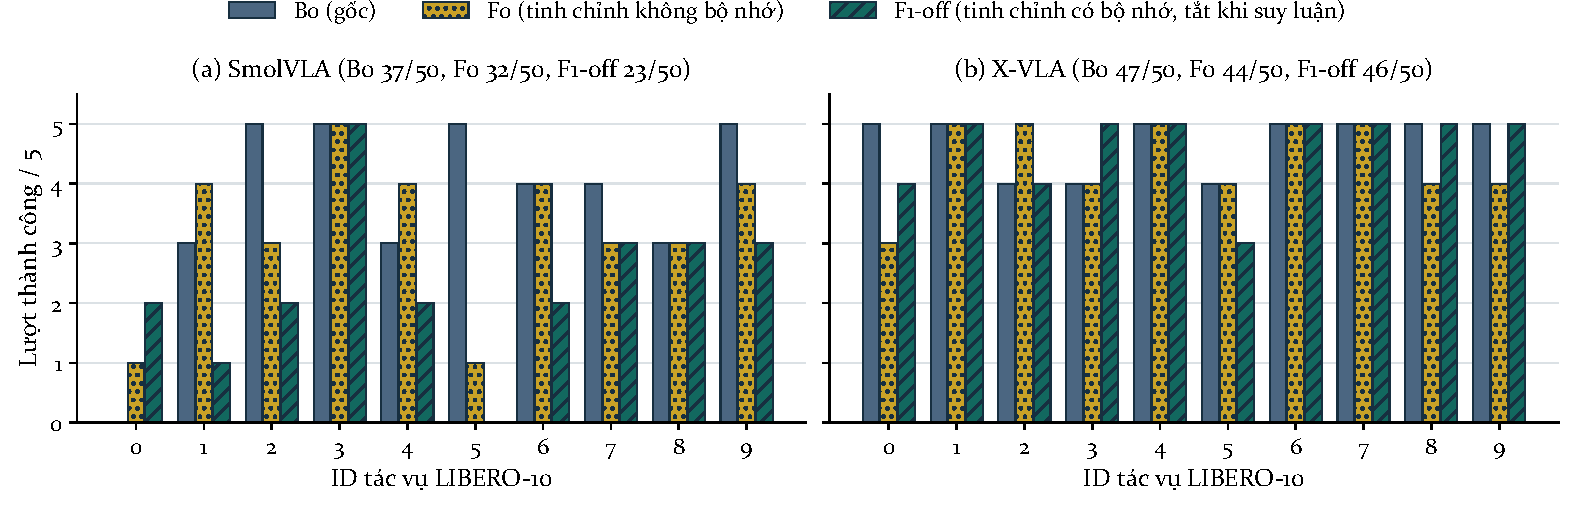
\includegraphics[width=.96\linewidth]{figures/duy-tri-e6.pdf}
\caption{Số lượt thành công theo từng tác vụ LIBERO-10 của B0, F0 và F1-off trên SmolVLA và X-VLA}
\label{fig:e6-retention-by-task}
\end{figure}

\section{Tổng hợp kết quả theo câu hỏi nghiên cứu}
\label{sec:ch4-rq-summary}

\textbf{RQ1: Giá trị của bộ nhớ sự kiện.} Đánh giá vòng kín cho thấy việc đưa dữ kiện bộ nhớ vào lời nhắc ngôn ngữ tác động trực tiếp đến động học ra quyết định nhưng chưa đủ để tự động nâng cao tỷ lệ thành công nếu thiếu cơ chế kiểm soát chu kỳ. Trên SmolVLA, F1 đạt 0 trên 40 lượt so với 4 trên 40 lượt của F0; trên X-VLA, cả hai cấu hình đạt 0 trên 40 lượt do lỗi lặp thao tác thừa, mặc dù F1 đạt tỷ lệ hoàn thành mốc SCR cao hơn rõ rệt với $0{,}492$ so với $0{,}350$. Thử nghiệm can thiệp triệt tiêu tại một truy vấn khẳng định chính sách nhạy bén ở mức cục bộ với sự hiện diện của đoạn văn bản ghi nhớ. Giá trị thực tế then chốt của bộ nhớ sự kiện được thể hiện rõ nét khi đóng vai trò nguồn bằng chứng định lượng cho cơ chế dừng ngoại vi: khi thay thế bằng các thời điểm dừng ngẫu nhiên, số lượt hoàn thành tác vụ sụt giảm mạnh từ 9 lượt xuống mức trung bình $3{,}7$ trên 40 lượt.

\textbf{RQ2: Độ tin cậy của bằng chứng và hiệu quả của cơ chế dừng.} Nghiên cứu đã chứng minh tính khả thi và hiệu quả rõ rệt của cơ chế điều phối theo sự kiện cùng giải pháp can thiệp dừng dựa trên bằng chứng bộ nhớ. Trong điều khiển vòng kín, bộ điều phối theo sự kiện vận hành chính xác theo thiết kế, ngắt thành công các đoạn hành động mở đoạn khi môi trường xuất hiện chuyển pha thao tác để kích hoạt mô hình tái truy vấn sớm. Đáng chú ý, nghiên cứu làm sáng tỏ bản chất của hiện tượng lặp thao tác thừa: X-VLA đạt tỷ lệ hoàn thành mốc SCR lên tới $0{,}833$ nhưng lại vượt quá chu kỳ quy định ở $83{,}3$\% số lượt chạy của tác vụ T1 do chính sách thiếu khả năng tự kết thúc nhiệm vụ. Cơ chế dừng ngoại vi kết hợp giữa bộ ghi thị giác và cảm nhận bản thể đã giải quyết triệt để điểm nghẽn này, nâng tỷ lệ thành công thực tế của X-VLA từ 0 trên 40 lên 9 trên 40 lượt trong vòng kín thật, gồm 8 trên 20 lượt ở tác vụ T1 và 1 trên 20 lượt ở tác vụ T3. Toàn bộ các lần dừng đúng lúc đều đạt kết quả thành công tuyệt đối và không phát sinh trường hợp dừng non gây hại. Trên nhóm phát triển 12 trạng thái seen, cùng cấu hình mang lại bước nhảy vọt từ 0 lên 6 trên 12 lượt thành công với ý nghĩa thống kê vững chắc ở mức $p = 0{,}031$. Việc tích hợp tín hiệu cảm nhận bản thể đã bù đắp hiệu quả độ trễ và sự che khuất của thị giác, thiết lập một quy trình xác thực bằng chứng tin cậy cho điều khiển thao tác dài hạn.

\textbf{RQ3: Duy trì kỹ năng cơ sở và khả năng thích ứng kiến trúc.} Khóa luận đã kiểm chứng thành công khả năng chuyển giao của khung phương pháp bộ nhớ sự kiện trên hai kiến trúc VLA có nguyên lý vận hành hoàn toàn khác biệt. Cùng một quy trình tạo dữ liệu, chiếu ngôn ngữ và huấn luyện tinh chỉnh đã được triển khai đồng bộ trên cả SmolVLA và X-VLA. Về khả năng duy trì kỹ năng cơ sở trên LIBERO-10, mức độ ảnh hưởng của quá trình tinh chỉnh có sự phân hóa sâu sắc giữa hai cấu hình mô hình: SmolVLA F1-off sụt giảm 28 điểm phần trăm từ 74\% xuống 46\%, trong khi X-VLA thể hiện khả năng bảo toàn tri thức vượt trội khi duy trì mức 92\% so với 94\% của checkpoint gốc, với mức chênh lệch nhỏ chưa mang ý nghĩa thống kê trên cỡ mẫu 50 cặp ghép. Điều kiện F0 của SmolVLA đạt 64\%, không khác biệt rõ với B0 nhưng cao hơn F1-off 18 điểm phần trăm, nên trên giao thức cục bộ một seed này, phần lớn mức suy giảm của SmolVLA gắn với việc huấn luyện trên lời nhắc bộ nhớ hơn là với bản thân việc tinh chỉnh.

Các kết quả thực nghiệm trong chương này củng cố vững chắc Đóng góp 2 về tính vận hành của kiến trúc bộ nhớ sự kiện có bằng chứng và Đóng góp 3 về quy trình đánh giá đa tầng từ mô phỏng cục bộ đến điều khiển vòng kín thực tế. Chương 5 sẽ tổng kết toàn bộ khóa luận, nêu rõ các giới hạn còn tồn tại và đề xuất các định hướng nghiên cứu tiếp theo.
